\section{Advies om machine learning toe te passen}

\subsection{Debugging}

Wanneer we ons model testen met nieuwe data, zou het kunnen dat er grote fouten in de voorspellingen zitten. Er zijn een grote verscheidenheid aan zaken die we kunnen proberen om dit op te lossen:
\begin{itemize}
	\item Meer trainingsdata toevoegen
	\item Minder \textit{features} gebruiken
	\item Meer \textit{features} gebruiken
	\item Extra polynomiale \textit{features} toevoegen
	\item $\lambda$ kleiner maken
	\item $\lambda$ groter maken
\end{itemize}
\noindent
Een diagnostiek is een test die we kunnen runnen om inzicht te krijgen in wat er wel of niet werkt binnen ons model en hoe we dit best kunnen verbeteren. In dit hoofdstuk zullen we enkele manieren bekijken. 

\subsection{Training, validatie en test sets}

We kunnen onze dataset opdelen in 3 delen, namelijk een training set, een cross-validatie set en een test set. De training set zal gewoonlijk uit 60$\%$ van onze dataset bestaan en zal gebruikt worden om het model te trainen. De cross-validatie set (ook wel \textit{development set}) bestaat gewoonlijk uit 20$\%$ van de dataset en wordt gebruikt om de hyperparameters te tunen. De test set bestaat uit de overige 20$\%$ en zal gebruikt worden om het model te testen met onafhankelijke data. \\
\newline
Om de performantie van ons model te onderzoeken, zullen we naar de kostfunctie zonder regularisatie kijken. Dit levert ons de volgende trainings -, cross-validatie - en testfout op, die we natuurlijk zo klein mogelijk willen houden:
\begin{equation}
	J_{train} = \frac{1}{2m} \sum_{i=1}^{m} (f_{\vec{w},b} (\vec{x}^{(i)}) - y^{(i)})^{2}
\end{equation}
\begin{equation}
	J_{CV} = \frac{1}{2m_{CV}} \sum_{i=1}^{m_{CV}} (f_{\vec{w},b} (\vec{x}^{(i)}) - y^{(i)})^{2}
\end{equation}
\begin{equation}
	J_{test} = \frac{1}{2m_{test}} \sum_{i=1}^{m_{test}} (f_{\vec{w},b} (\vec{x}^{(i)}) - y^{(i)})^{2}
\end{equation}
\noindent
Wanneer we nu een aantal modellen hebben die bestaan uit veeltermen van een bepaalde graad, kunnen we gaan kijken wel model het meest geschikt is voor ons probleem door altijd onze kostfunctie te minimaliseren. We kunnen de gevonden parameters vervolgens gebruiken om de trainingsfout en cross-validatiefout te berekenen. De trainingsfout zal kleiner worden naarmate de graad van ons model groter wordt. Dit is echter niet het geval voor de cross-validatiefout. Deze zal ergens een optimaal minimum hebben. We zijn op zoek naar het model waarbij dit het geval is, aangezien deze de kleinste fout heeft op ongeziene data. We kunnen vervolgens nog de gewichten van dit model gebruiken om de kost op onze test set te berekenen zodat we die kunnen rapporteren, maar dit gebeurt echter niet altijd in de literatuur. 

\subsection{\textit{Bias} en variantie diagnosticeren}

We kunnen de waarden voor $J_{train}$ en $J_{CV}$ ook linken aan eventuele \textit{over -} of \textit{underfitting} van het model. De trainingsfout zal heel groot zijn in het geval van \textit{underfitting} (\textit{high bias}) en heel klein zijn in het geval van \textit{overfitting} (\textit{high variance}). De cross-validatiefout zal een optimale waarde bereiken bij een robuust model en dus een grotere waarde hebben in het geval van \textit{high bias} of \textit{high variance}. Dit is ook zichtbaar op Figuur \ref{fig:error-plot}.

\begin{figure}[h]
	\centering
	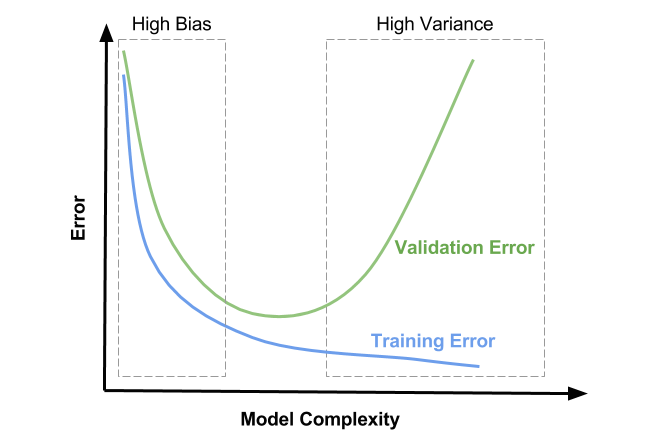
\includegraphics[width=0.65\linewidth]{images/18-error-plot.png}
	\caption{Visualisatie van training - en cross-validatiefout}
	\label{fig:error-plot}
\end{figure}

\subsection{\textit{Bias} en variantie regulariseren}

We kunnen ook de invloed van de regularisatieparameter $\lambda$ linken aan eventuele \textit{over -} of \textit{underfitting} van het model. Zoals we eerder al kort aangekaart hebben, is de functie van regularisatie het tegengaan van \textit{high variance}. Wanneer deze hyperparameter dus te klein is, hebben we te maken met \textit{overfitting} en wanneer $\lambda$ te groot is, hebben we te maken met \textit{underfitting}. Dit zien we op Figuur \ref{fig:error-plot-lambda}. 

\begin{figure}[h]
	\centering
	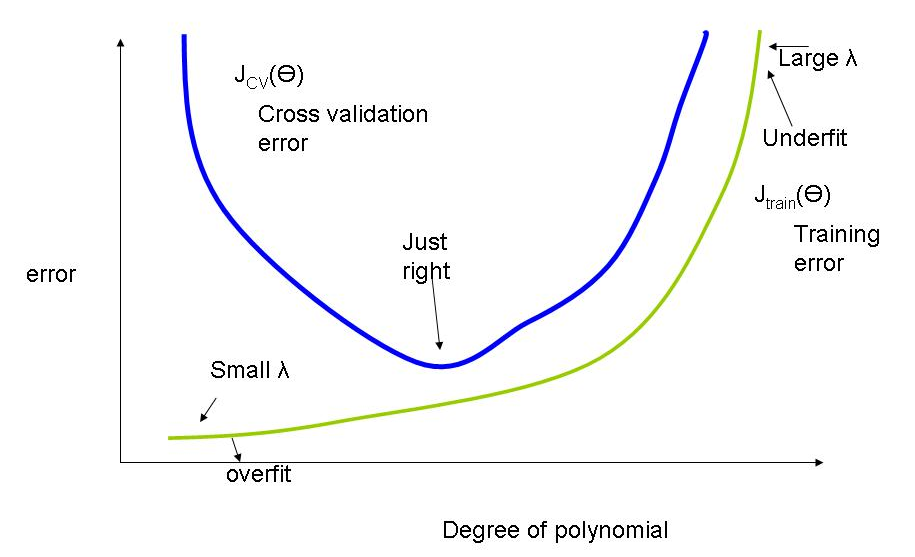
\includegraphics[width=0.65\linewidth]{images/19-error-plot-lambda.png}
	\caption{Visualisatie van training - en cross-validatiefout}
	\label{fig:error-plot-lambda}
\end{figure}
\noindent
We kunnen hier opnieuw een aantal modellen vergelijken, in dit geval allemaal getraind met een verschillende waarde voor de hyperparameter $\lambda$. Hierna zullen we op dezelfde manier de trainings - en crossvalidatiefout berekenen en op deze manier het meest geschikte model uitkiezen, namelijk die met de kleinste waarde voor $J_{CV}$. 

\subsection{Model selectie in neuraal netwerk}

Wanneer we kunnen kiezen uit een aantal  modellen met een verschillen aantal lagen en nodes, zullen we opnieuw de trainings - en cross-validatiefout berekenen en het model met de kleinste $J_{CV}$ kiezen. 

\subsection{Leercurves}

Leercurves (\textit{learning curves}) plotten de grootte van de trainings - en cross-validatiefout wanneer we de grootte van de training set doen toenemen. De groene curve op Figuur \ref{fig:learning-curves} stelt $J_{CV}$ voor en de blauwe curve is $J_{train}$. We zien dat $J_{train}$ toeneemt bij een toename van $m$, terwijl $J_{CV}$ afneemt. \\
\newline
In het geval van \textit{high bias}, zullen we een grote fout hebben op onze training - en cross-validatie set. Het toevoegen van extra trainingsdata zal hier niet helpen. Dit is bij \textit{high variance} wel het geval om de \textit{gap} tussen $J_{train}$ en $J_{CV}$ te doen afnemen.

\begin{figure}[h]
	\centering
	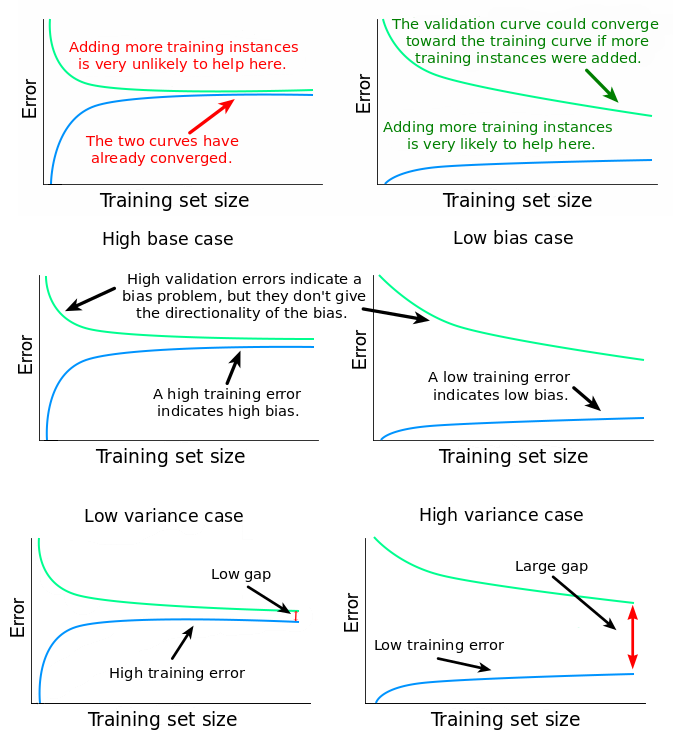
\includegraphics[width=0.65\linewidth]{images/20-learning-curves.png}
	\caption{Leercurves voor variantie en \textit{bias}}
	\label{fig:learning-curves}
\end{figure}

\subsection{\textit{Bias} en variantie tegengaan}

We kunnen dus concluderen dat wanneer we te maken hebben met \textit{high bias}, we dit kunnen oplossen door extra \textit{features} toe te voegen, extra polynomiale \textit{features} toe te voegen of de regularisatieparameter $\lambda$ te verkleinen. \textit{High variance} kan tegengegaan worden door meer trainingsdata toe te voegen, minder \textit{features} te gebruiken of de regularisatieparameter $\lambda$ te vergroten.